%% !TEX root =  paper.tex

\begin{figure*}[t]
\centering
\begin{subfigure}{\columnwidth}
\centering
%\fbox{
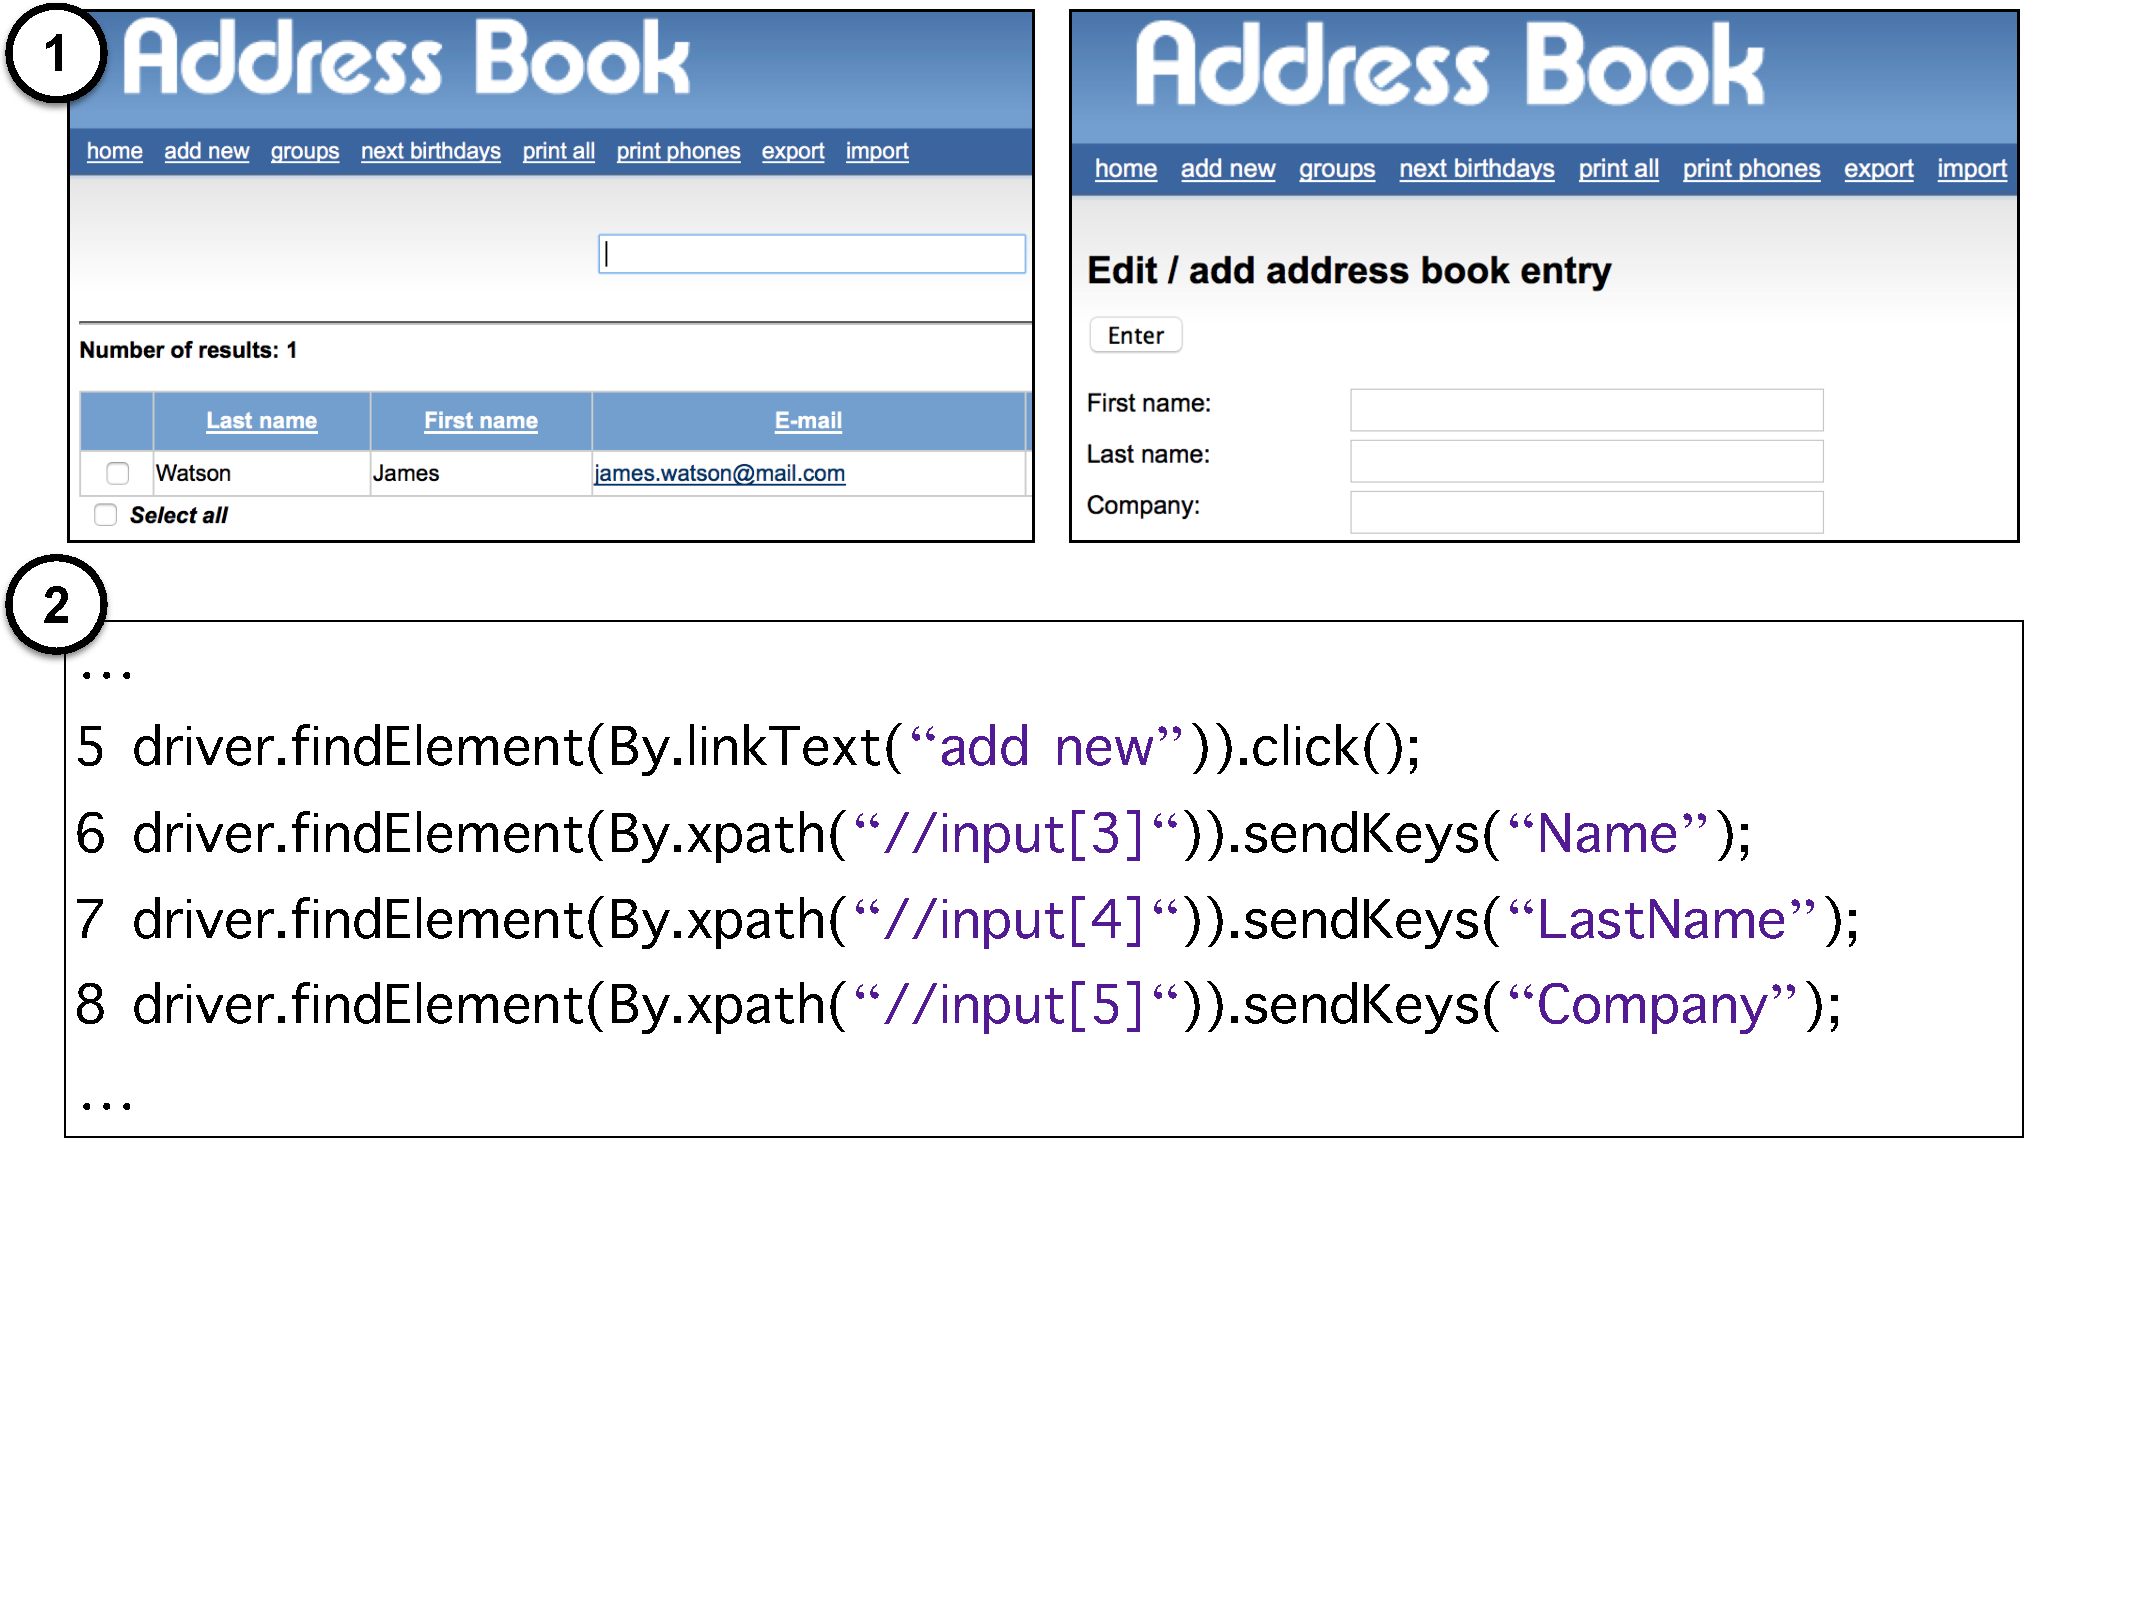
\includegraphics[trim=0cm 7.5cm 1.8cm 0cm, clip=true, scale=0.23]{images/addressbook-version1.pdf}
%}
\caption{\emph{Version 6.2.12}}
\label{fig:ab1} 
\end{subfigure}
\begin{subfigure}{\columnwidth}
\centering
%\fbox{
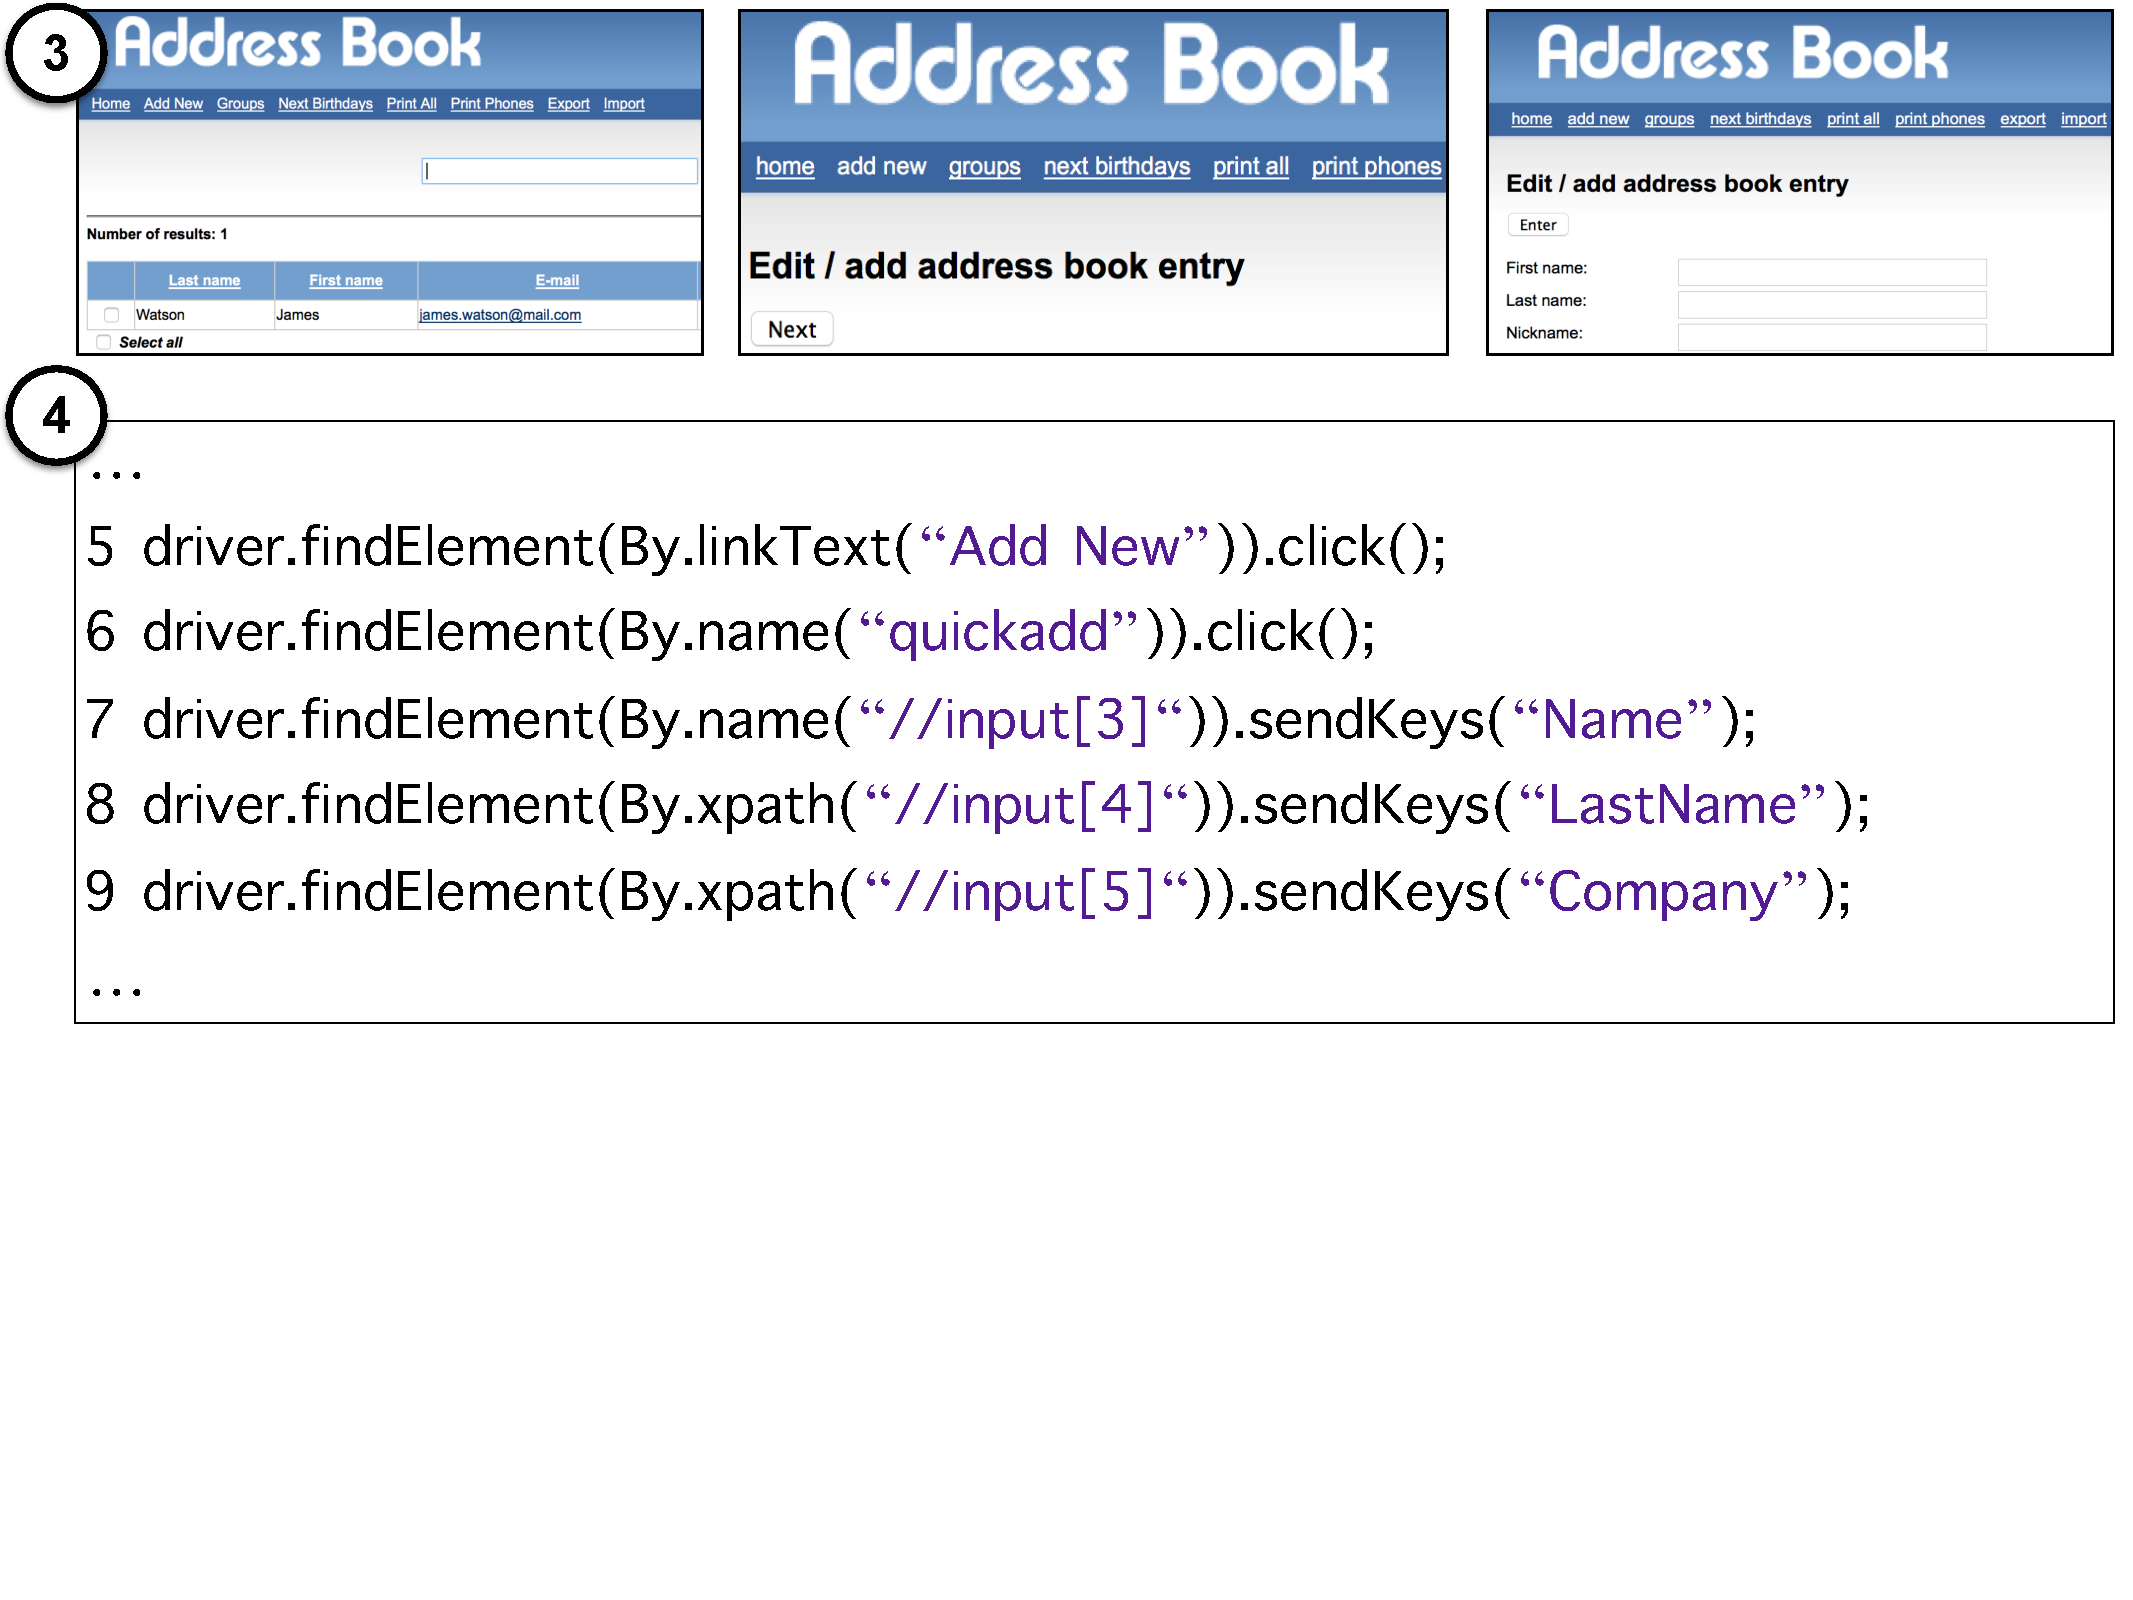
\includegraphics[trim=0cm 9.5cm 0cm 0cm, clip=true,  scale=0.260]{images/addressbook-version2.pdf}
%}
\caption{\emph{Version 7.0.0}}
\label{fig:ab2} 
\end{subfigure}
\caption{AddressBook web application, version 6.2.12 (\ref{fig:ab1}) and version 7.0.0 (\ref{fig:ab2}), along with  automated Selenium WebDriver tests. \andrea{find a way to show the web pages bigger}} 
\label{fig:example} 
\end{figure*}

\subsection{Breakage Scenarios}\label{sec:breakage-scenarios}

Given the predominance of locator-related issues, we focus our analysis on locator problems. In the following of this section, we present four (4) challenging test breakage scenarios, and we show how the visual analysis can help to mitigate or correct such problems. 

\noindent
\textbf{Basic Terminology.}
At a high level, each web test statement is a tuple \textit{<locator, action, value>}. 
The locator component specifies the web element the test statement is interacting with. A locator is a function on a DOM state $\mathcal{D}$. Notationally, $l: \mathcal{D} \rightarrow \{e\}$ where $e$ is the web element returned by the locator $l$ when applied to $\mathcal{D}$. 
%
%Locator breakages are due to one or more DOM-based root causes. A root cause is a tuple $<\mathcal{D}, e, a, v>$ where $\mathcal{D}$ is a DOM tree (e.g., a test state), $e$ is the web element in $\mathcal{D}$ on which the test currently operates, $a$ is a HTML attribute of $e$, and $v$ is the value of $a$. 
%We define a repair as a tuple $<r, e', a', v', \mathcal{D'}>$, where $r$ is a root cause and $e'$ is the suggested new web element for $\mathcal{D}$ in the root cause $r$, having attribute $a'$ set to $v'$. 
%The locator function is surjective, that is every web element $e$ is mapped to by at least one locator (e.g., the XPath from the root to $e$), but there exist multiple locators {$\displaystyle \forall l\in L,\exists e\in D{\text{ such that }} l: D \rightarrow \{e\}$}.

\noindent
\textbf{Scenario 1 (Non-Selection $\bullet$ Element Present Same State).}
A non-selection occurs when a locator $l$ applied to a DOM state $\mathcal{D}$ returns no elements---formally, $l: \mathcal{D} \rightarrow \emptyset$, but the target element $e$ is still present on the page ($e \in \mathcal{D}$).
Then, possible repairs require to find another locator $l'$, such that $l': \mathcal{D} \rightarrow e$.

As an example, consider the login page of AddressBook in~\autoref{fig:ab-back-a}, and the WebDriver test of ~\autoref{fig:ab-back-c}. %, which was developed for (or evolved until) version 6.2.12, where it runs correctly.
%\textcircled{\raisebox{-0.8pt}{1}}~shows the home page of AddressBook web application version 6.2.12, and the page in which the user can insert a new entry. A portion of a possible Selenium WebDriver test script is also shown~\textcircled{\raisebox{-0.8pt}{2}}, which was developed for (or evolved until) version 6.2.12, where it runs correctly.
%
Suppose in a new subsequent version of AddressBook (e.g., 7.0.0), as a result of the application evolution, the \texttt{id} of the ``Login'' button gets deleted, and the tag of the element modified (e.g., from \texttt{input} to \texttt{button}). 
%\texttt{id=``submitLogin''}. In particular, the menu bar items have been capitalized, and a new confirmation page has been added before the insert entry page. 
%Finally,~\textcircled{\raisebox{-0.9pt}{4}} shows a portion of a Selenium WebDriver test~\cite{selenium} which fills in the username and password input boxes (Lines~5-6), and submits the form (Line~7). Suppose the test was developed for (or evolved until) version 1.10.0, where it ran correctly.
When executed on version 7.0.0~\textcircled{\raisebox{-0.8pt}{3}}, the test will then stop when attempting to locate the ``Login'' button. Non-selection problems manifest as \textit{direct} breakages, because the broken statement is the one that needs to be repaired.  
%
At a visual inspection of the two GUIs, a tester would expect the test to work, because her perception is immaterial where changes at DOM-level are concerned. It is indeed evident that the target element is \textit{visually} still present on the page, and its position \textit{on the GUI} has not changed.
 
%This is a simple instance of \textit{test breakage}, because the test scenario is unaltered, and no bugs are (eventually) present in the application. However, the automated test ceases to be applicable because it has lost the synchronization with the AUT, and a repair needs to be found.
At this aim, a tester may wish to use the \water  technique~\cite{Choudhary:2011:WWA:2002931.2002935} to automatically repair the broken statement. Specifically, another locator for the ``Login'' button needs to be found, rather the relying on ``broken'' attribute \texttt{id}. \water will attempt to gather information about the broken element (such as the XPath, and the various attributes) by analysing the DOM of the previous version, and match such information on the evolved DOM of version 7.0.0. Unfortunately, \water's technique is ineffective in such a scenario, because (1)~the attribute \texttt{id} has been deleted from the DOM, and (2)~the XPath and the tag of the target element have changed (from \mbox{\texttt{input}} to \mbox{\texttt{button}}), which renders impossible for \water's heuristic to identify it on the evolved DOM. % and apply its automatic repair.
 
\noindent
\textit{Visual-aided Mitigation.}
In this case, an algorithm taking into consideration the visual appearance of the test state might be able to match the target element between the two GUIs (in a similar way as a human would do). However, this task is challenging to be automated because several issues needs first to be solved. Among all (1)~finding an accurate visual matching technique, and, in the case a visual match is found, (2)~retrieving the corresponding element in the DOM. 

\noindent
\textbf{Scenario 2 (Non-Selection $\bullet$ Element Moved to Neighbouring State).}
As a concrete example consider \autoref{fig:ab1}, showing Addressbook web application version 6.2.12~\textcircled{\raisebox{-0.7pt}{1}}, specifically the pages in which the user can insert a new entry. The test~\textcircled{\raisebox{-0.7pt}{2}} clicks on the ``add new'' link on the home page (Line~5), and fills in the First name, Last name and Company text fields (Lines~6--8).
Suppose now to replay the test on the successive version 7.0.0~\textcircled{\raisebox{-0.7pt}{3}}, for regression purposes. The test will raise an exception of kind \texttt{NoSuchElementException} at Line~6, when attempting to locate the ``First name'' text field~\textcircled{\raisebox{-0.7pt}{2}}. 
Indeed, a new intermediate confirmation page has been added~\textcircled{\raisebox{-0.9pt}{3}}, and the navigational workflow of the test must be corrected to reflect that of the new modified web application.

From a testing perspective, the ``First name'' text field can no longer be found on the web page (test state) following the execution of the statement at Line~5. However, conceptually, the repair action that needs to be triggered in order to correct the test has nothing to do with the locator at Line~6.
In fact, by only looking at the exception, it is arduous for the tester to understand what the problem is, unless the \textit{visual execution} of the test is taken into consideration.
%
Even the use of \water is unsuccessful, because it would attempt at repairing the broken statement at Line~6. (the technique only handles addition of statements within forms, and does not apply to general broken workflow scenarios).

\noindent
\textit{Visual-aided Mitigation.}
A possible solution would require to (1)~detect that the web element $e$ no longer exists as part of the test state $st_i$ in version $V$, (2)~try to match the $e$ in one of the neighbouring states of $st_i$ in the new version $V'$, which requires to (3)~find  a web element $e' \in st_i$ such that $(e', st_i) \rightarrow st_j$ (the ``Next'' button in our example~\textcircled{\raisebox{-0.7pt}{3}}).

\noindent
\textbf{Scenario 3 (Non-Selection $\bullet$ Element Absent).} 
%
The third and last non-selection scenario presented concerns a web element being deleted from a web page. In a way, this can be seen as the opposite scenario of Scenario 2. 
As a concrete example, consider the example of \autoref{fig:ab2}, with the application being evolved in the reverse order as depicted in the figure (thus considering going from version 7.0.0 to version 6.2.12). The test~\textcircled{\raisebox{-0.7pt}{4}} would stop at Line 6, when trying to select the ``Next'' button, which was on a page that is no longer present. In this case, the only possible fix is to delete the statement.

\noindent
\textit{Visual-aided Mitigation.}
A possible solution would require to (1)~search for the the web element $e$ both in $st_i$ and its neighbouring states, and (2)~if not match is found, then remove the statement.

\noindent
\textbf{Scenario 4 (Mis-Selection).}\label{sec:misselection}
Problems occur not only when web elements are being deleted, but also when they get modified, either in their position on the DOM tree, or in their position in the application state space. This can cause tests to ``mis-select'' elements.
Specifically, a mis-selection occurs when a locator selects a different DOM element from the one that was used to target. 
%Suppose having version $V$ and a test $t$, composed of a statement $st_i$, which uses a locator $l$ (where $l: \mathcal{D} \rightarrow \{e\}$). In the next version $V'$, $l: \mathcal{D}' \rightarrow \{e'\}$ where $e \ne e'$.
Notationally, $l: \mathcal{D} \rightarrow \{e\}$ in $V$, and $l: \mathcal{D}' \rightarrow \{e'\}$ in $V'$ where $e \ne e'$.
%A mis-selection of an element can lead to unpredictable misbehaviours of the test, being responsible of either direct or propagated breakages.

Consider \autoref{fig:example} again. 
Suppose that the test~\textcircled{\raisebox{-0.9pt}{2}} is repaired so as to reach the edit page on version 7.0.0 (for instance, as in~\textcircled{\raisebox{-0.9pt}{4}}). On the new version 7.0.0, the statements at Lines~6--7 will execute correctly, whereas at Line~8 (which will be Line~9 in the new version) will fill in the field Nickname, instead of the field Company. %In literature, this is known as mis-selection problem~\cite{Choudhary:2011:WWA:2002931.2002935}.
 
The mis-selection problem can lead to unpredictable test executions, that diverge from the test's intended behaviour. Depending on the kind of actions, the test execution might result in a direct, propagated or silent breakage~\cite{Hammoudi-2016-ICST}. Typically, the test continues its execution until it reaches a point in which an action cannot be performed or an element cannot be found, but the actual repair has to be triggered \textit{in a previous test statement}.

\noindent
\textit{Visual-aided Mitigation.}
A possible solution would require to (1)~visually validate that the web element $e$ is still targeting the correct element in the new version and (2)~try to correct it, otherwise.

\noindent
\textbf{Summary.}
We have presented four (4) test breakage scenarios and we have discussed how the visual appearance of the SUT can be utilized to overcome the existing test repair approaches and give an important contribution to the tester. We do not claim, however, that such a list represents all the possible scenarios. It is worth remarking that the context is further complicated by the fact that the presented scenarios can occur together (i.e., leading to \textit{multiple} breakages in the same test), which complicates detecting and repair activities even further.

%\head{How Testers Repair}
%%
%%When a test $t$ that was used to function on a version $V$  breaks on a successive version $V'$, a tester needs to understand the root cause behind the breakage and a possible repair for it. 
%%
%When a test $t$ breaks, at least four steps are involved. 
%(1)~The tester inspects the error stack trace or the console, which may contain information about the origin of breakage (e.g., ``\texttt{NoSuchElementException} occurred. Unable to locate element with \mbox{\texttt{name=password}}''). 
%(2)~The tester uses the message to inspects $t$ looking for the statement $st$ responsible for the failure. %which is also likely to be the one that needs to be corrected (note that this is not always true).
%(3)~The tester navigates the GUI of $V'$, trying to identify the portion of the GUI related to $st$. 
%(4)~The tester inspects either the DOM, or the GUI, or both the DOM and the GUI of $V'$ to find candidate repair solutions. In doing so, the tester may possibly need to exercise manually the same broken scenario of $t$ (i.e., all the actions in the statements preceding $st$), in order to replicate the breakage occurred at $st$ and gather insights on possible repair actions.
%
%To wrap up, a \textbf{first challenge} in repairing web tests derives from the fact that  
%%Thus, in E2E web tests such as Selenium's 
%the tester often needs to inspect and link the behaviour of the test code execution, to the modification perpetrated to the GUI and the DOM of the application. 
%In other words, breakages are often repaired by finding candidate solutions through the inspection of the DOM and the GUI \textit{at the same time}.
%For this reason, it is arguably more difficult to repair Selenium's tests than standard JUnit tests for desktop applications (for which the error messages are typically more informative and IDE features make the debugging activities easier).
%%
%A \textbf{second challenge} is related to the time needed to find and correct the breakages, which may be significantly high~\cite{Leotta-TAIC-2013,JAMAICA2013}. One of the main reasons is due to the low support by the existing test automation tools in understanding the root causes behind test breakages and how they do relate with the changes made in the web applications. 
%
%In this paper we wish to make step ahead to provide such understanding. 
%Our aim is to combine the knowledge present in the DOM of the application with its visual appearance, so as to effectively aid the tester in detecting and repairing test breakages or in validating their correctness. %Our approach aims at automating the mental model the testers create when a test case is executed against a web application GUI. In our belief, such a model is a viable means for automating test case repair.

%Existing locator repair techniques are indeed limited when the web application undergoes drastic structural changes because they only consider the DOM as source where to find possible repairs.
%However, we argue that visual image recognition can help verify each test step (i.e., locator), signalling and fixing the breakages that pertain to locators.

\subsection{Brief Computer Vision Background}\label{sec:cv}

One of our motivations of conducting this research is to use computer vision (CV) techniques to assist software-engineering tasks. 
%In particular, we aim to propose a method that mimics how a user sees a web page, and how she decides whether an element is present or not, or it is the same on which it has interacted with in a previous execution. 
Thereby, we provide a short background of the CV solutions that are useful in our setting.

\noindent
\textbf{Template Matching.}\label{sec:tm}
Identifying web elements \textit{visually} across different versions (i.e., pages) of a web application falls within a common branch of image analysis known as template matching. 
%
Template matching aims to detect the occurrence of a specific  object image (template) in another image~\cite{Brunelli:2009:TMT:1643435}. The template is slid over the image, and a a similarity measure is computed at each pixel location
%This is done by defining a small image of the object, a template, and searching for a similar occurrence in a given image, by sliding the template over the image, and computing a similarity measure at each pixel location.
%
Template matching algorithms must account for factors such as scaling, rotation, and lighting. Fortunately, the images we aim to match in this work are screen captures from web applications rendered by the same browser. In this context, the above issues are ameliorated, and the main problems are, for instance, the shifting of GUI elements or the fact that some elements are not displayed at all~\cite{}.
% 
However, standard template matching algorithms are not effective in detecting the presence/absence of a template. Indeed, by design, they always return the pixel location where the best match has been found. Even if a stricter threshold value on the similarity coefficient might be used, in practice this is not robust or generalizable, thus we explored key-point matching.

\noindent
\textbf{Feature Detection.}
The philosophy of this method is to find certain ``important'' points (key-points) in the object template and store information about the neighbourhood of those key-points (key-point descriptors) as a description of the object. In other test images, one should find key-point descriptors of key-points in the whole image and try to `match' the two descriptor sets (one from the object template and one from the test image) using some notion of similarity, and see how many descriptors match.



